\section{DESARROLLO} 

\subsection{Desarrollo del Sistema}
\begin{enumerate}[1.]
	\item Pasos de desarrollo de la aplicacion
	\begin{enumerate}[a)]
	\item Paso 1: Diagrama de Clases de solución Cajero
		\begin{figure}[H]
		\begin{center}
		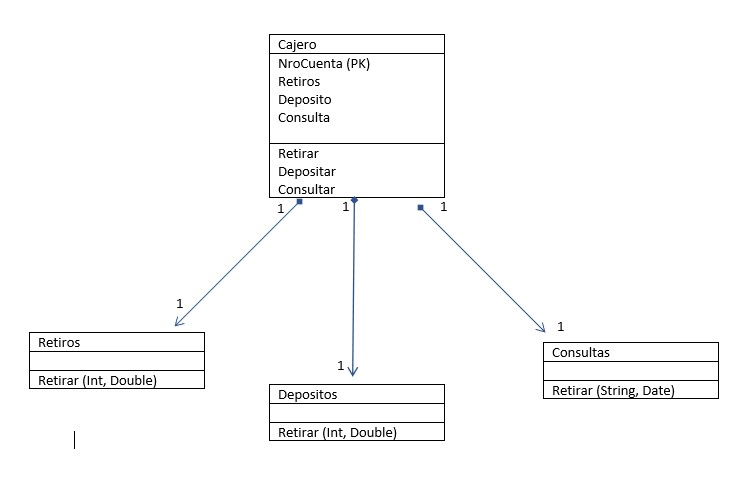
\includegraphics[width=8cm]{./Imagenes/img1}
		\end{center}
		\end{figure}
	\item Paso2: Crear un Windows form para desorrallar nuestra aplicación de escritorio:
		\begin{figure}[H]
		\begin{center}
		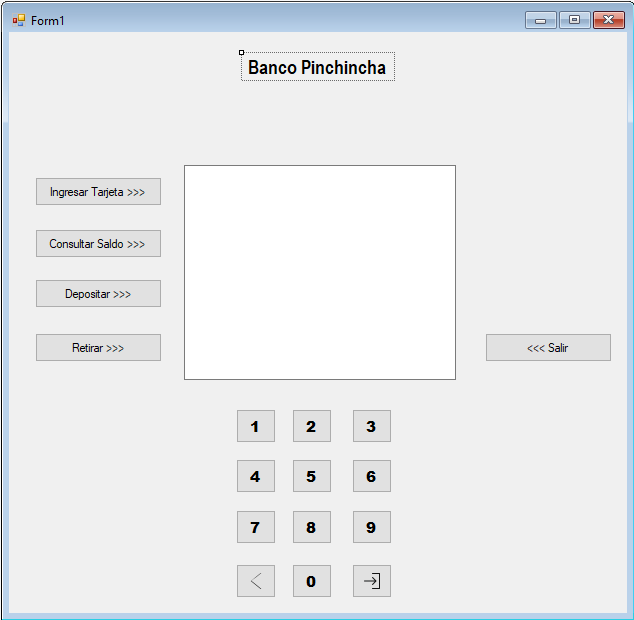
\includegraphics[width=6cm]{./Imagenes/img2}
		\end{center}
		\end{figure}
	\item Paso 3: Codificar los botones según lo planeado para nuestra aplicación, por ejemplo para esta aplicación hemos decidido 		virtualizar un cajero automático. \\
		\begin{figure}[H]
		\begin{center}
		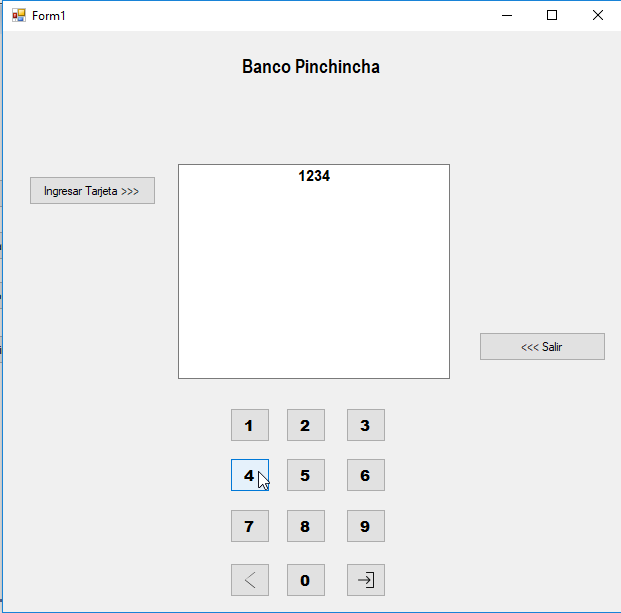
\includegraphics[width=7cm]{./Imagenes/img3}
		\end{center}
		\end{figure}
	\item Paso 4: Muestra de algo de código de los botones: 
		\begin{figure}[H]
		\begin{center}
		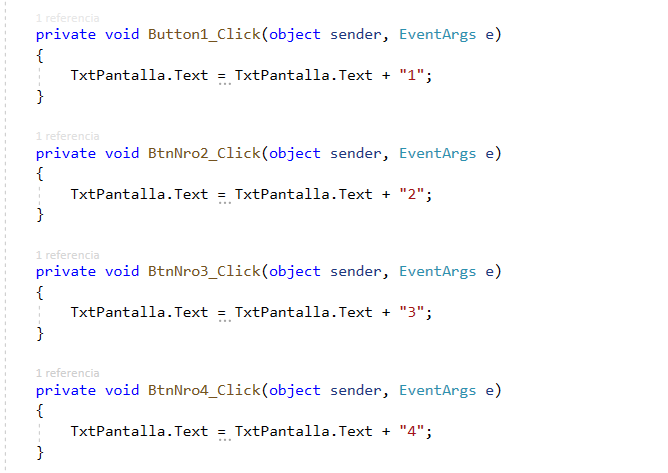
\includegraphics[width=6cm]{./Imagenes/img4}
		\end{center}
		\end{figure}
	\item Paso 5: aplicar un ORM a nuestra aplicación: aplicaremos el ORM Entity framework(define que es y para que sirve  entity framework) 
		\begin{figure}[H]
		\begin{center}
		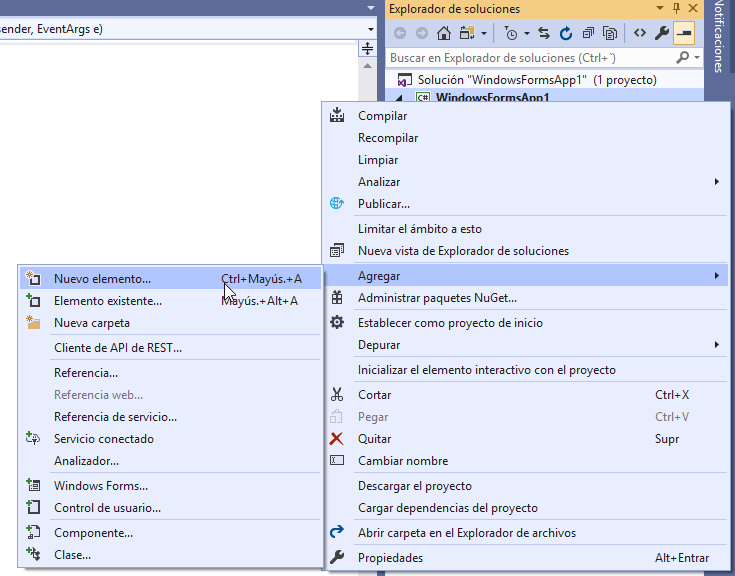
\includegraphics[width=7cm]{./Imagenes/img5}
		\end{center}
		\end{figure}
	\item Paso 6: Agregaremos el modelo ADO.NET entity data model
		\begin{figure}[H]
		\begin{center}
		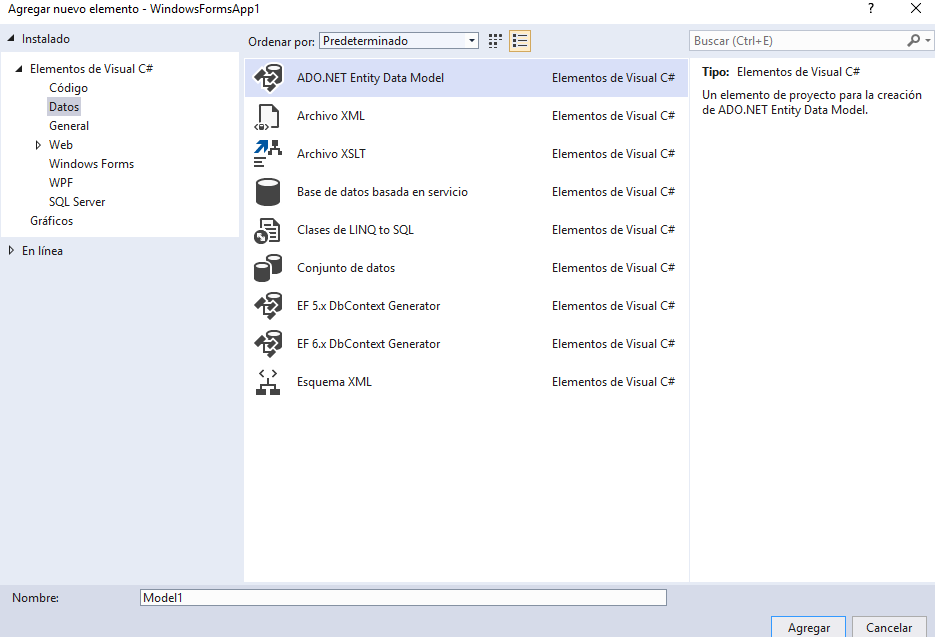
\includegraphics[width=7cm]{./Imagenes/img6}
		\end{center}
		\end{figure}
	\item Paso 7: ELuego configuraremos con la base de datos que se encuentra en Nuestro servidor SQL 
		\begin{figure}[H]
		\begin{center}
		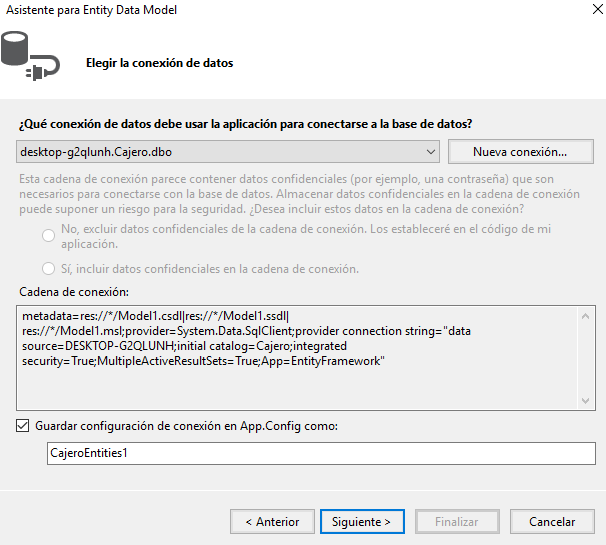
\includegraphics[width=8cm]{./Imagenes/img7}
		\end{center}
		\end{figure}
	\end{enumerate}

	\item Escribiendo consultas con el operador UNPIVOT
	\begin{enumerate}[a)]
	\item Paso 1: Crear y consultar la vista Sale.PivotCustGroups.\\
		-  Escribir la siguiente consulta para crear una vista llamada Sales.PivotCustGroups.\\
		\begin{figure}[H]
		\begin{center}
		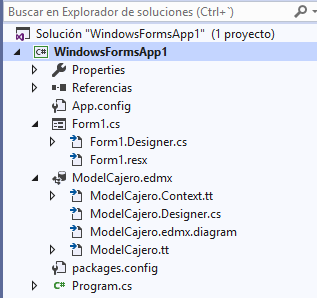
\includegraphics[width=8cm]{./Imagenes/img8}
		\end{center}
		\end{figure}
		-  Despues escribrir la siguiente consulta.
		\begin{figure}[H]
		\begin{center}
		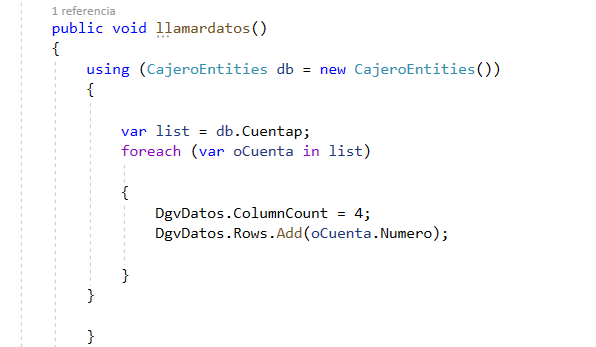
\includegraphics[width=5cm]{./Imagenes/img9}
		\end{center}
		\end{figure}
	\item Paso 2: Escriba una instruccion SELECT para recuperar una fila para cada pais y grupo de cliente.\\
		-  En el panel de consulta escribir la siguiente consulta.\\
		\begin{figure}[H]
		\begin{center}
		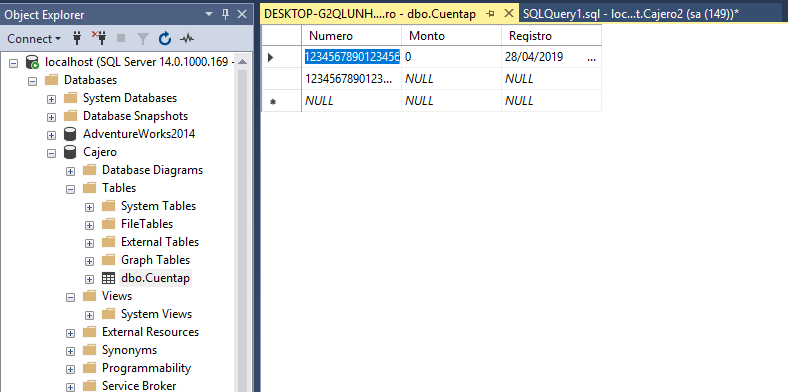
\includegraphics[width=7cm]{./Imagenes/img10}
		\end{center}
		\end{figure}
	\item Paso 3: Eliminar las vistas creadas.
		\begin{figure}[H]
		\begin{center}
		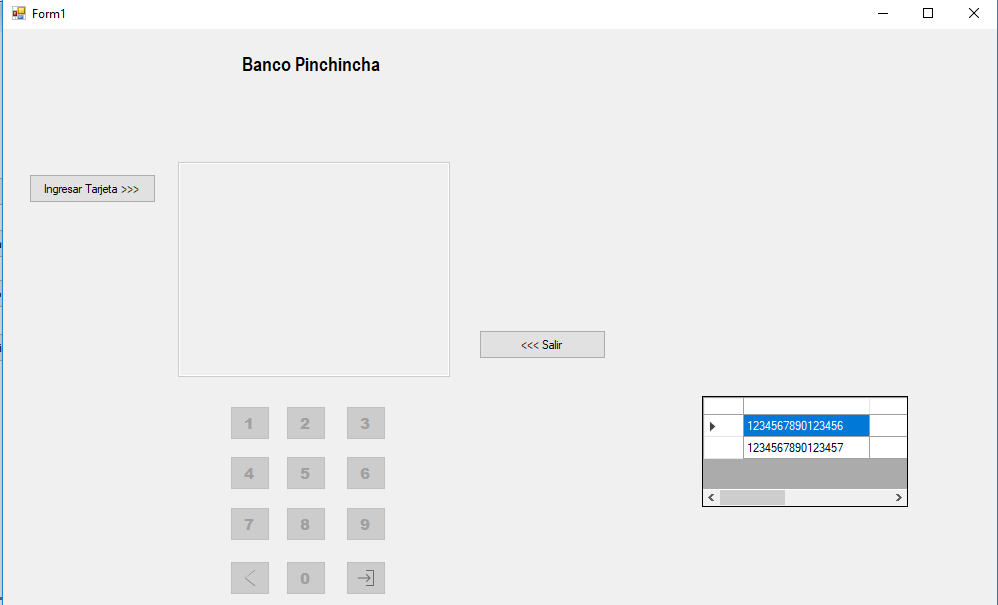
\includegraphics[width=6cm]{./Imagenes/img11}
		\end{center}
		\end{figure}
	\end{enumerate}



	\item Escribiendo consultas con las clausulas GROUPING SETS, CUBE, and ROLLUP.
	\begin{enumerate}[a)]
	\item Paso 1: Escriba una instruccion SELECT que use LA SUBCLAUSULA GROUPING SETS para devolver el número de
Clientes para diferentes conjuntos de agrupación.\\
		-  Escribir la siguiente consulta y ejecutar. 
		\begin{figure}[H]
		\begin{center}
		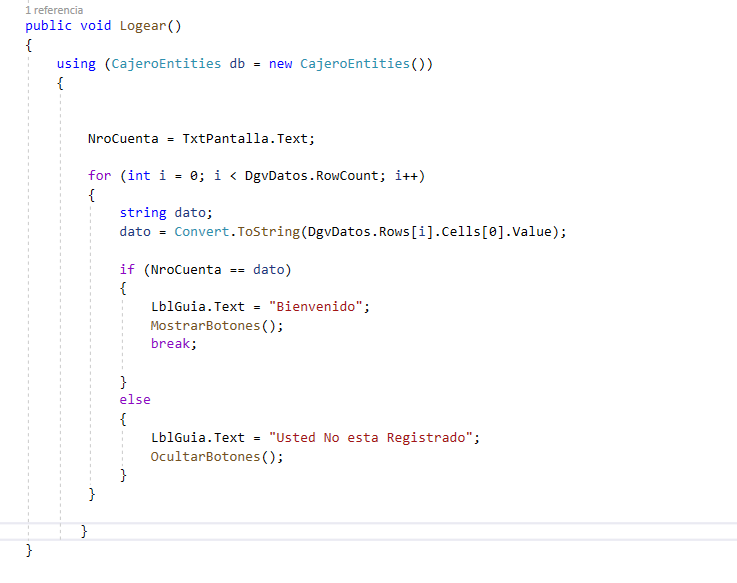
\includegraphics[width=7cm]{./Imagenes/img12}
		\end{center}
		\end{figure}
	\item Paso 2: Escriba una instruccion SELECT que use la subclausula CUBE para recuperar Grouping sets basados en valores de ventas anuales, mensuales y diarios.\\
		-  Escribir la siguiente consulta. 
		\begin{figure}[H]
		\begin{center}
		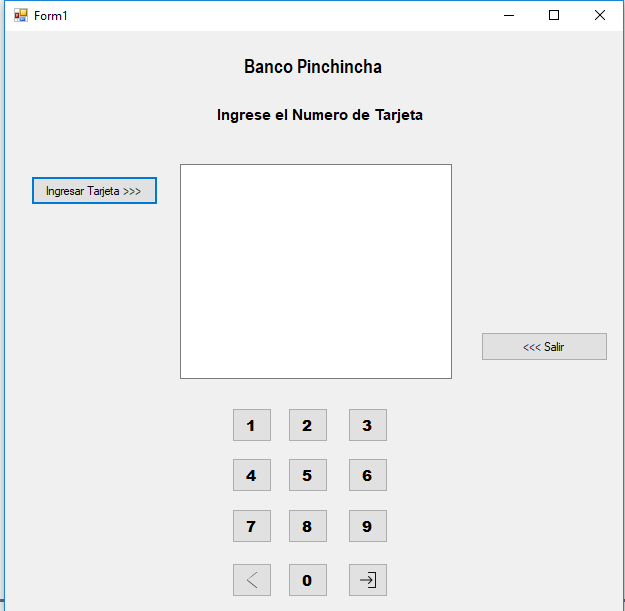
\includegraphics[width=7cm]{./Imagenes/img13}
		\end{center}
		\end{figure}
	\item Paso 3: Escriba la misma instruccion SELECT usando la subclausula ROLLUP.\\
		-  Escribir la siguiente consulta. 
		\begin{figure}[H]
		\begin{center}
		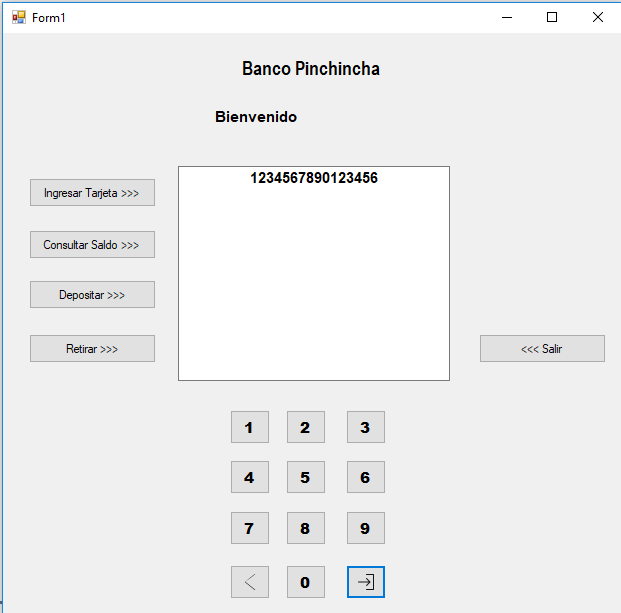
\includegraphics[width=7cm]{./Imagenes/img14}
		\end{center}
		\end{figure}
	\item Paso 4: Analizar el valor total de ventas por año y mes.\\
		-  Escribir la siguiente consulta y ejecutar. 
		\begin{figure}[H]
		\begin{center}
		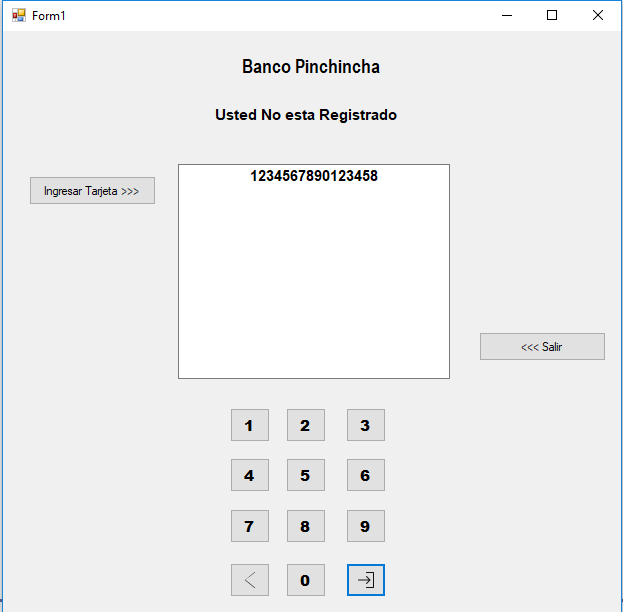
\includegraphics[width=7cm]{./Imagenes/img15}
		\end{center}
		\end{figure}
	\end{enumerate}
\end{enumerate}

\subsection{Analisis}
\begin{enumerate}[1.]
	\item Escribiendo consultas con el operador PIVOT
	\begin{enumerate}[a)]
	\item Paso 1: Escribir una sentencia SELECT para recuperar el numero de clientes para un grupo especifico de clientes.\\
		-  Abrir el SQL Server Management Studio y conectar a la basa de datos (local) usando Windows.\\
		-  Usar la base de datos TSQL\\
		-  Ejecutar el siguiente codigo para crear una vista\\
		\begin{figure}[H]
		\begin{center}
		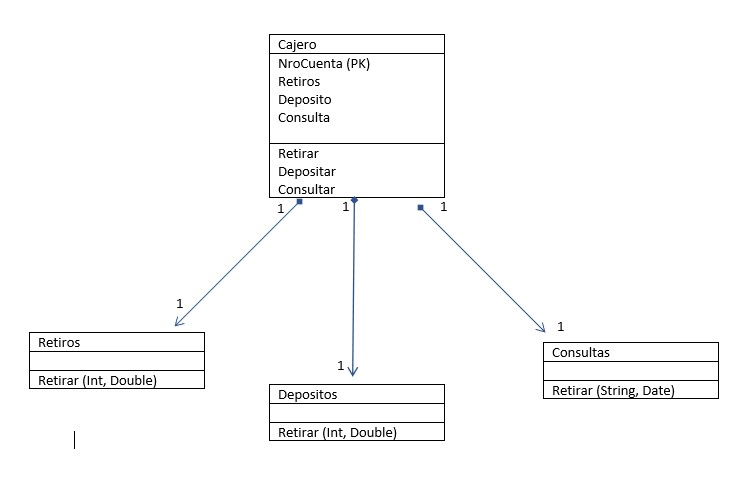
\includegraphics[width=8cm]{./Imagenes/img1}
		\end{center}
		\end{figure}
		-  En el panel de consulta, escribir la siguiente consulta.
		\begin{figure}[H]
		\begin{center}
		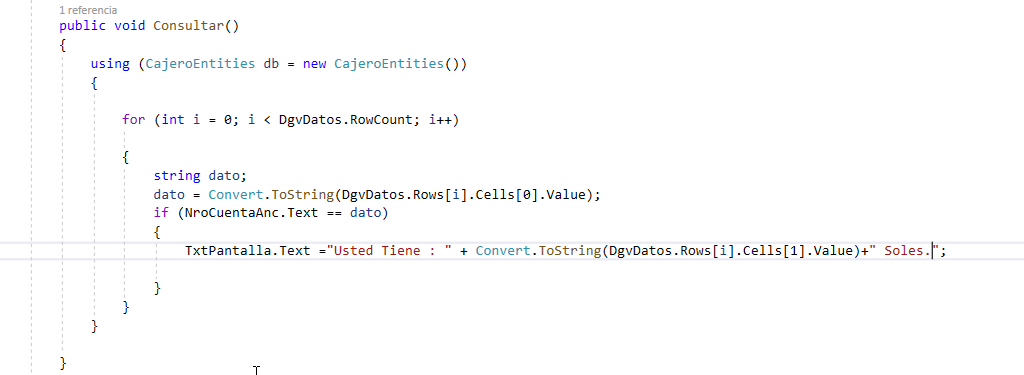
\includegraphics[width=6cm]{./Imagenes/img16}
		\end{center}
		\end{figure}
		-  Luego modificamos el codigo, aplicando el operador PIVOT.
		\begin{figure}[H]
		\begin{center}
		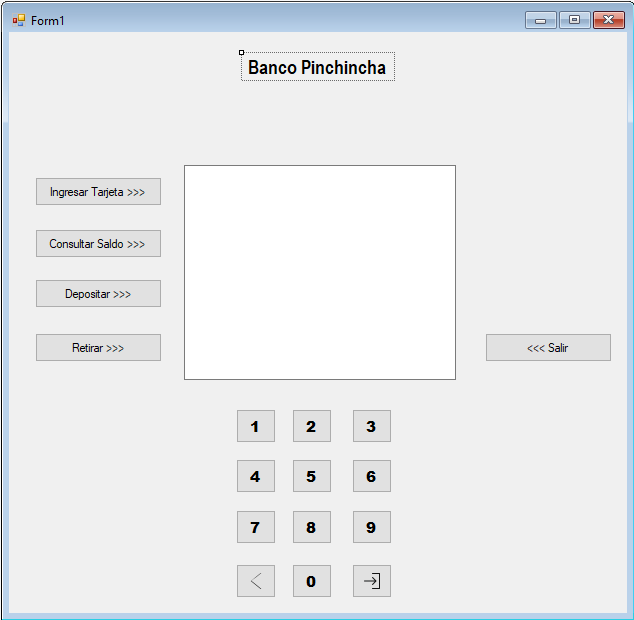
\includegraphics[width=6cm]{./Imagenes/img2}
		\end{center}
		\end{figure}
	\item Paso 2: Especifique el elemento de agrupacion para el operador PIVOT. \\
		-  Escribir la siguiente consulta para poder modificar la vista creada anteriormente, añadiendo 2 columnas adicionales. 
		\begin{figure}[H]
		\begin{center}
		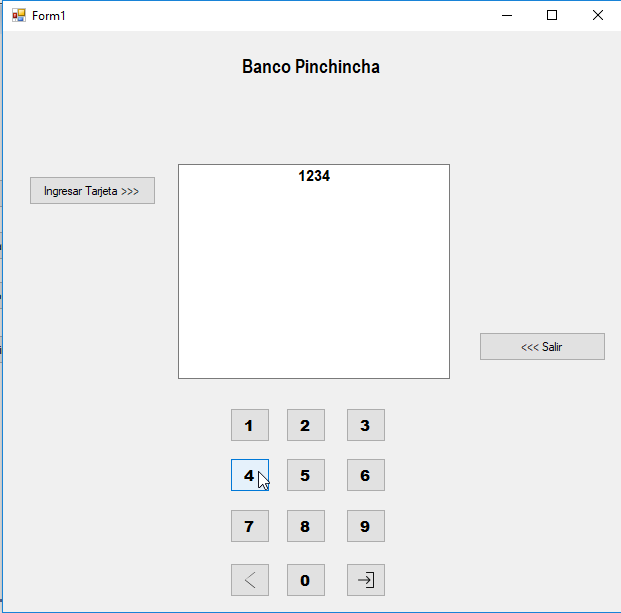
\includegraphics[width=7cm]{./Imagenes/img3}
		\end{center}
		\end{figure}
		-  Escribir la siguiente consulta. 
		\begin{figure}[H]
		\begin{center}
		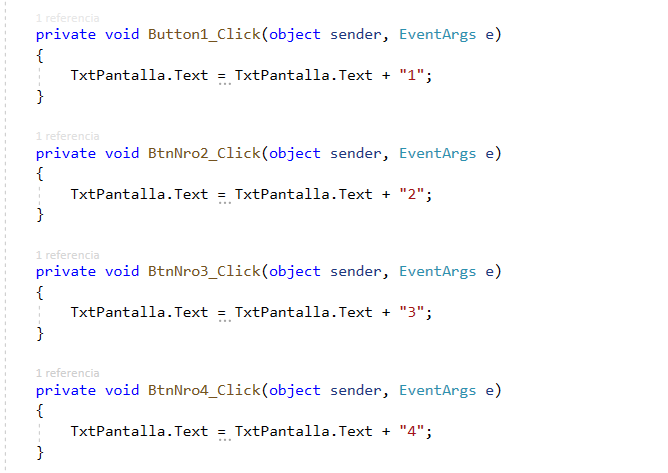
\includegraphics[width=6cm]{./Imagenes/img4}
		\end{center}
		\end{figure}
		-  Modificar la consulta para incluir columnas adicionales desde la vista. 
		\begin{figure}[H]
		\begin{center}
		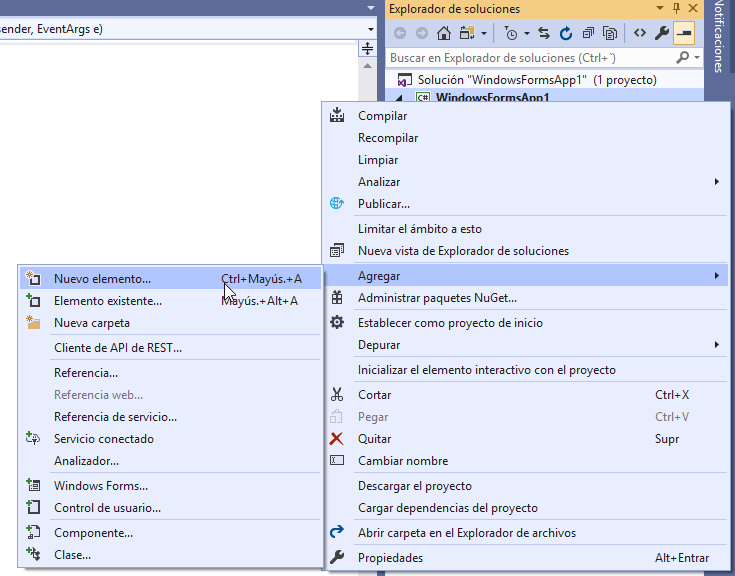
\includegraphics[width=7cm]{./Imagenes/img5}
		\end{center}
		\end{figure}
	\item Paso 3: Use una expresion de tabla común (CTE) para especificar el elemnto de agrupacion para el operador PIVOT.\\
		-  Escribir la siguiente consulta y ejecutar. 
		\begin{figure}[H]
		\begin{center}
		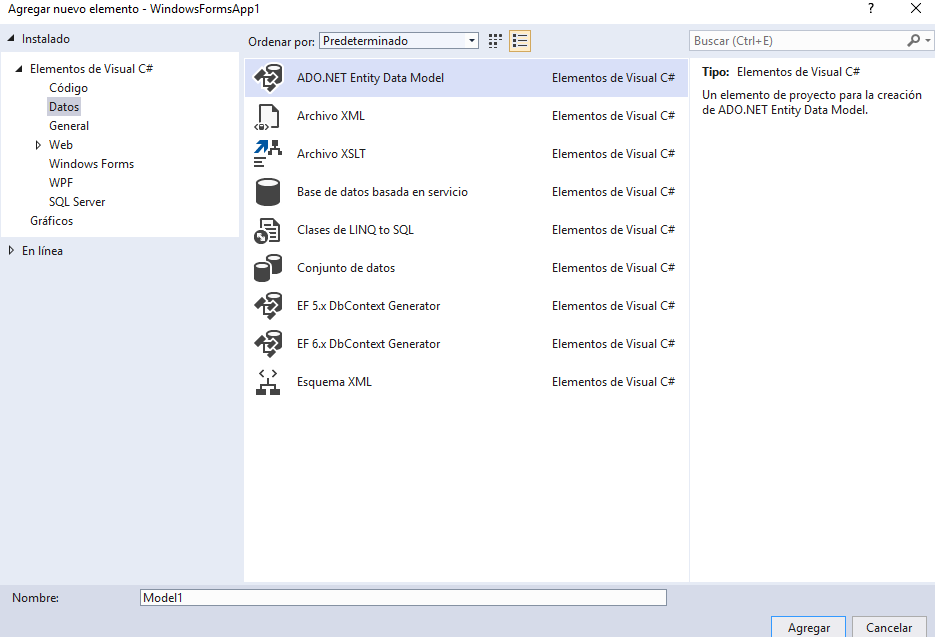
\includegraphics[width=7cm]{./Imagenes/img6}
		\end{center}
		\end{figure}
	\item Paso 4: Escribe una instruccion SELECT para recuperar el monto total de ventas para cada cliente y categoria de producto.\\
		-  Escribir la siguiente consulta. 
		\begin{figure}[H]
		\begin{center}
		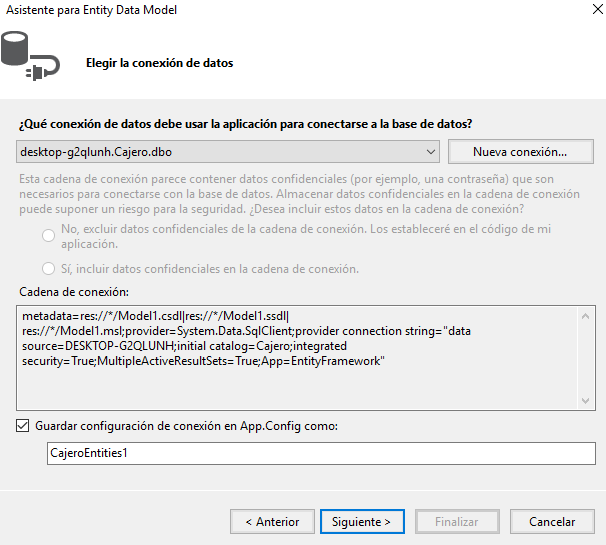
\includegraphics[width=8cm]{./Imagenes/img7}
		\end{center}
		\end{figure}
	\end{enumerate}

	\item Escribiendo consultas con el operador UNPIVOT
	\begin{enumerate}[a)]
	\item Paso 1: Crear y consultar la vista Sale.PivotCustGroups.\\
		-  Escribir la siguiente consulta para crear una vista llamada Sales.PivotCustGroups.\\
		\begin{figure}[H]
		\begin{center}
		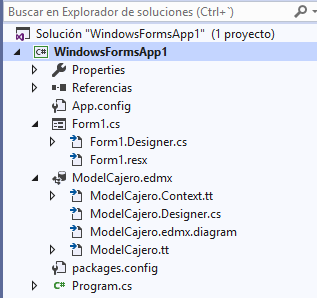
\includegraphics[width=8cm]{./Imagenes/img8}
		\end{center}
		\end{figure}
		-  Despues escribrir la siguiente consulta.
		\begin{figure}[H]
		\begin{center}
		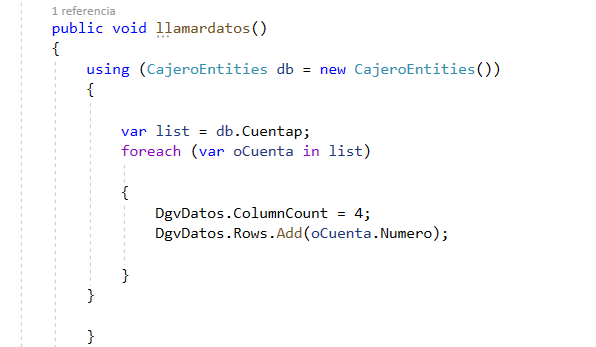
\includegraphics[width=5cm]{./Imagenes/img9}
		\end{center}
		\end{figure}
	\item Paso 2: Escriba una instruccion SELECT para recuperar una fila para cada pais y grupo de cliente.\\
		-  En el panel de consulta escribir la siguiente consulta.\\
		\begin{figure}[H]
		\begin{center}
		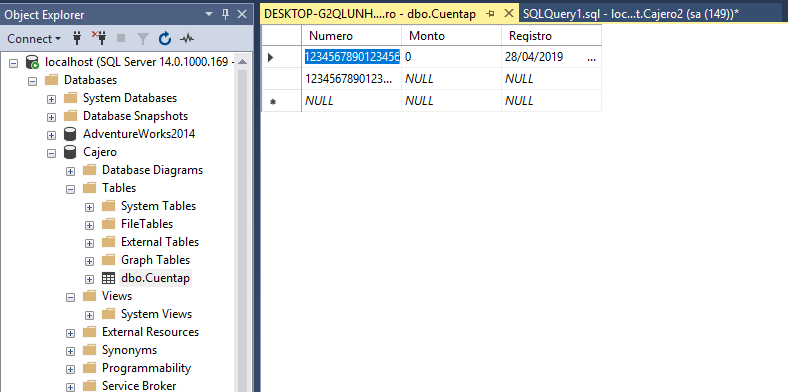
\includegraphics[width=7cm]{./Imagenes/img10}
		\end{center}
		\end{figure}
	\item Paso 3: Eliminar las vistas creadas.
		\begin{figure}[H]
		\begin{center}
		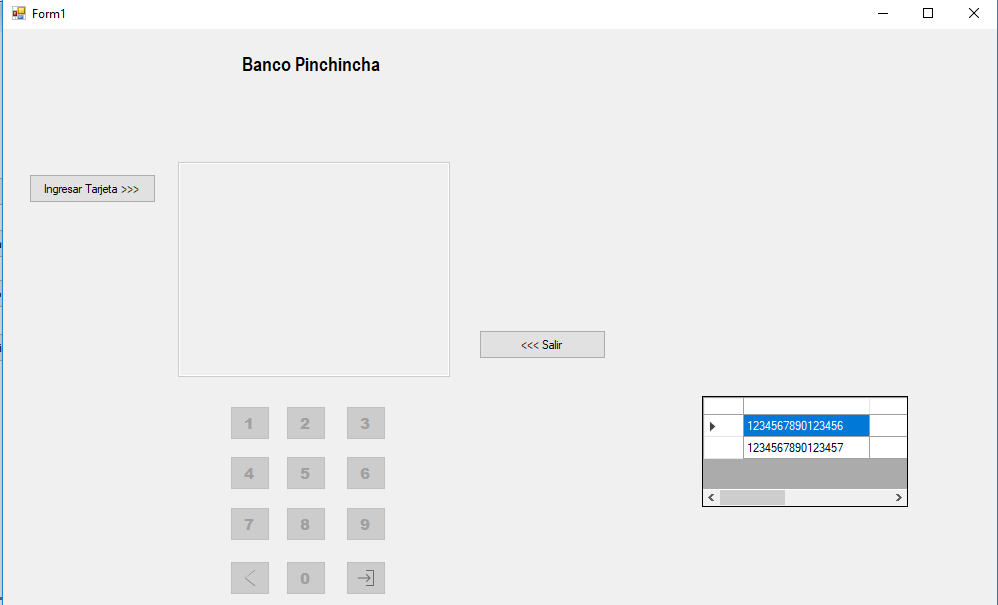
\includegraphics[width=6cm]{./Imagenes/img11}
		\end{center}
		\end{figure}
	\end{enumerate}



	\item Escribiendo consultas con las clausulas GROUPING SETS, CUBE, and ROLLUP.
	\begin{enumerate}[a)]
	\item Paso 1: Escriba una instruccion SELECT que use LA SUBCLAUSULA GROUPING SETS para devolver el número de
Clientes para diferentes conjuntos de agrupación.\\
		-  Escribir la siguiente consulta y ejecutar. 
		\begin{figure}[H]
		\begin{center}
		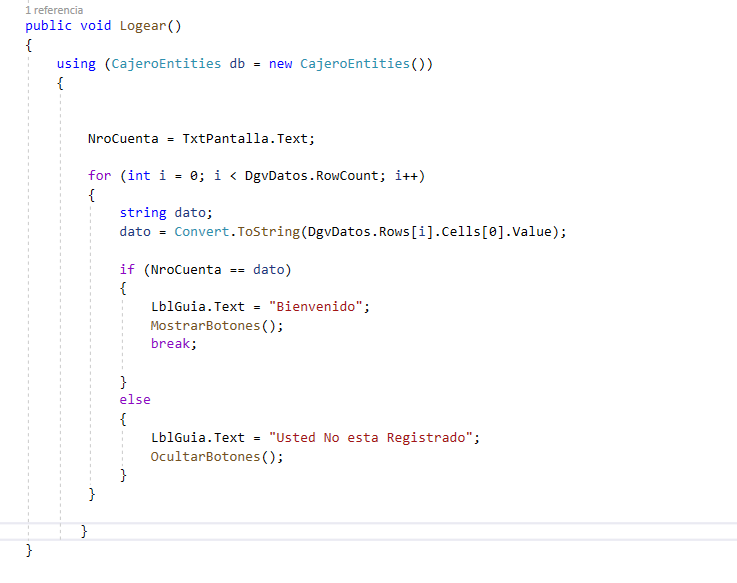
\includegraphics[width=7cm]{./Imagenes/img12}
		\end{center}
		\end{figure}
	\item Paso 2: Escriba una instruccion SELECT que use la subclausula CUBE para recuperar Grouping sets basados en valores de ventas anuales, mensuales y diarios.\\
		-  Escribir la siguiente consulta. 
		\begin{figure}[H]
		\begin{center}
		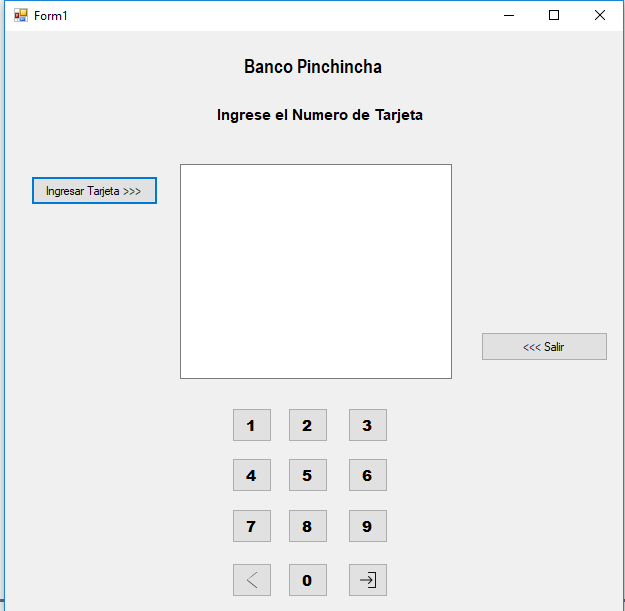
\includegraphics[width=7cm]{./Imagenes/img13}
		\end{center}
		\end{figure}
	\item Paso 3: Escriba la misma instruccion SELECT usando la subclausula ROLLUP.\\
		-  Escribir la siguiente consulta. 
		\begin{figure}[H]
		\begin{center}
		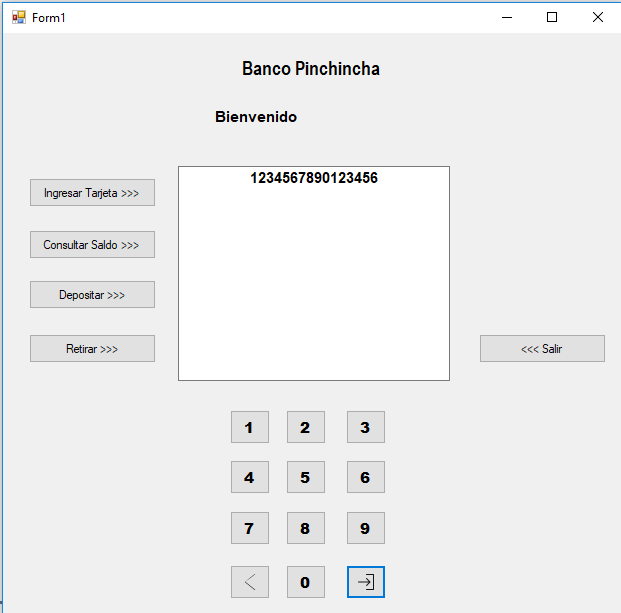
\includegraphics[width=7cm]{./Imagenes/img14}
		\end{center}
		\end{figure}
	\item Paso 4: Analizar el valor total de ventas por año y mes.\\
		-  Escribir la siguiente consulta y ejecutar. 
		\begin{figure}[H]
		\begin{center}
		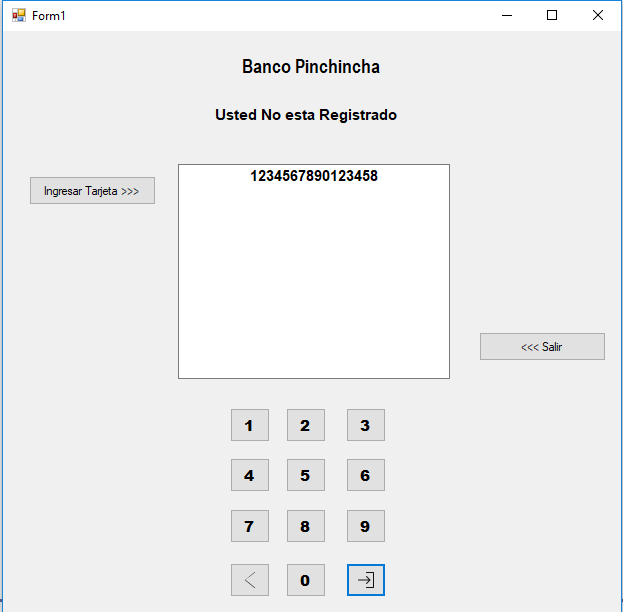
\includegraphics[width=7cm]{./Imagenes/img15}
		\end{center}
		\end{figure}
	\end{enumerate}
\end{enumerate}

	
\subsection{Diseño}
\begin{enumerate}[1.]
	\item Escribiendo consultas con el operador PIVOT
	\begin{enumerate}[a)]
	\item Paso 1: Escribir una sentencia SELECT para recuperar el numero de clientes para un grupo especifico de clientes.\\
		-  Abrir el SQL Server Management Studio y conectar a la basa de datos (local) usando Windows.\\
		-  Usar la base de datos TSQL\\
		-  Ejecutar el siguiente codigo para crear una vista\\
		\begin{figure}[H]
		\begin{center}
		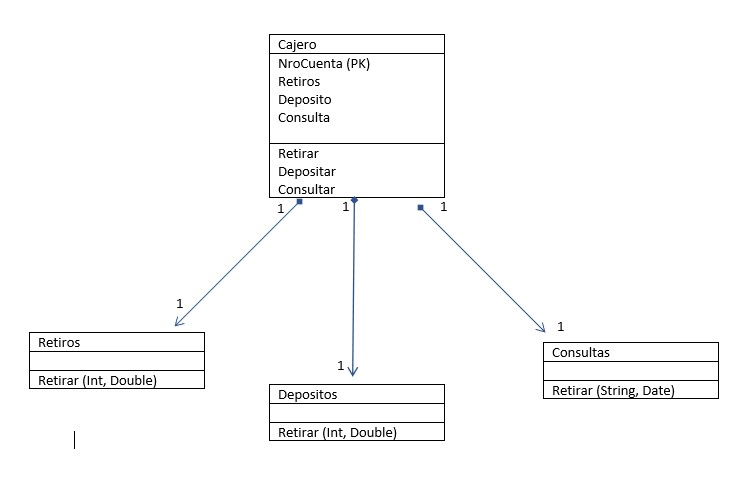
\includegraphics[width=8cm]{./Imagenes/img1}
		\end{center}
		\end{figure}
		-  En el panel de consulta, escribir la siguiente consulta.
		\begin{figure}[H]
		\begin{center}
		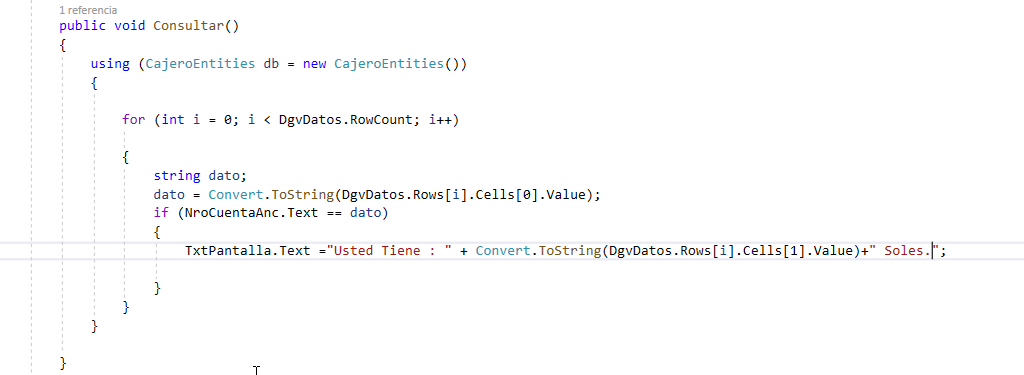
\includegraphics[width=6cm]{./Imagenes/img16}
		\end{center}
		\end{figure}
		-  Luego modificamos el codigo, aplicando el operador PIVOT.
		\begin{figure}[H]
		\begin{center}
		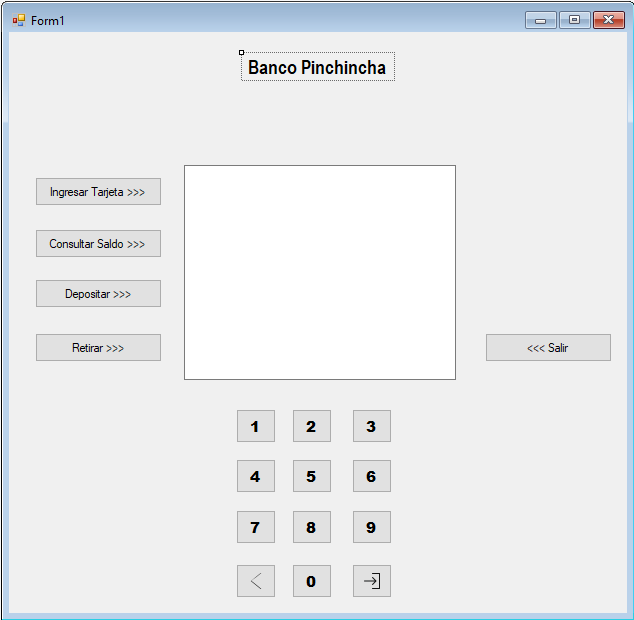
\includegraphics[width=6cm]{./Imagenes/img2}
		\end{center}
		\end{figure}
	\item Paso 2: Especifique el elemento de agrupacion para el operador PIVOT. \\
		-  Escribir la siguiente consulta para poder modificar la vista creada anteriormente, añadiendo 2 columnas adicionales. 
		\begin{figure}[H]
		\begin{center}
		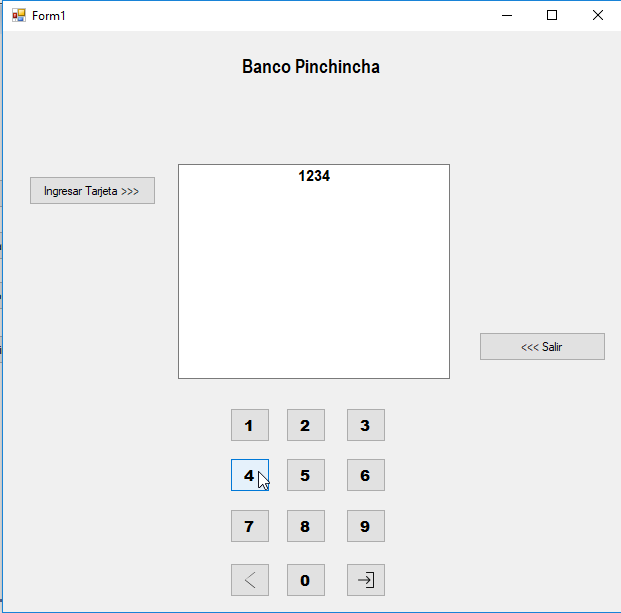
\includegraphics[width=7cm]{./Imagenes/img3}
		\end{center}
		\end{figure}
		-  Escribir la siguiente consulta. 
		\begin{figure}[H]
		\begin{center}
		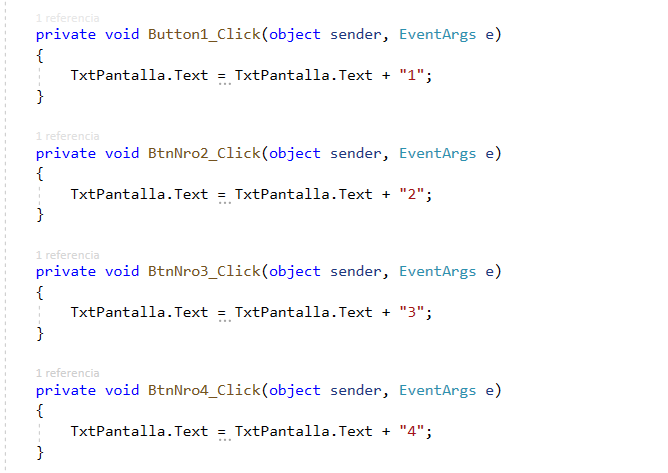
\includegraphics[width=6cm]{./Imagenes/img4}
		\end{center}
		\end{figure}
		-  Modificar la consulta para incluir columnas adicionales desde la vista. 
		\begin{figure}[H]
		\begin{center}
		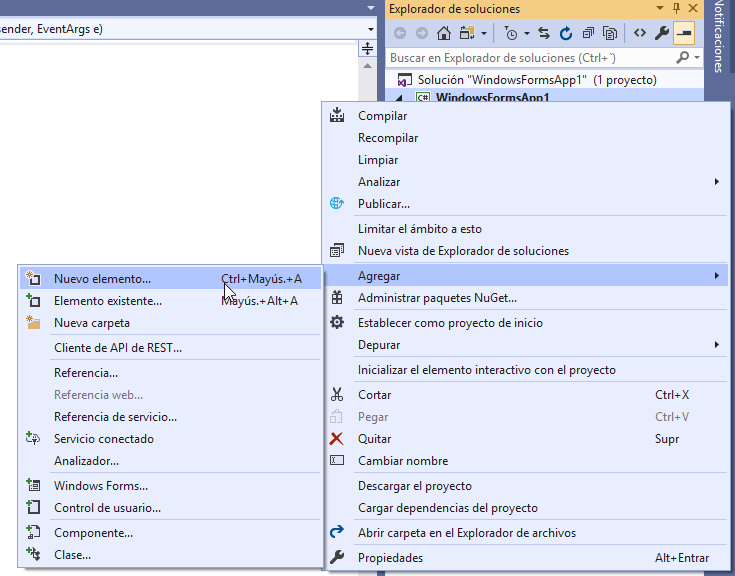
\includegraphics[width=7cm]{./Imagenes/img5}
		\end{center}
		\end{figure}
	\item Paso 3: Use una expresion de tabla común (CTE) para especificar el elemnto de agrupacion para el operador PIVOT.\\
		-  Escribir la siguiente consulta y ejecutar. 
		\begin{figure}[H]
		\begin{center}
		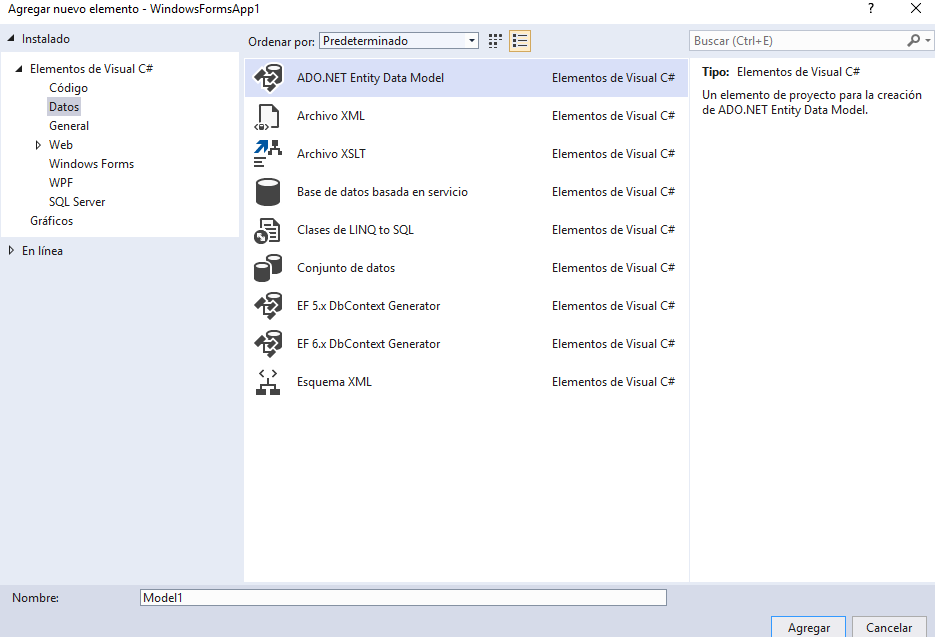
\includegraphics[width=7cm]{./Imagenes/img6}
		\end{center}
		\end{figure}
	\item Paso 4: Escribe una instruccion SELECT para recuperar el monto total de ventas para cada cliente y categoria de producto.\\
		-  Escribir la siguiente consulta. 
		\begin{figure}[H]
		\begin{center}
		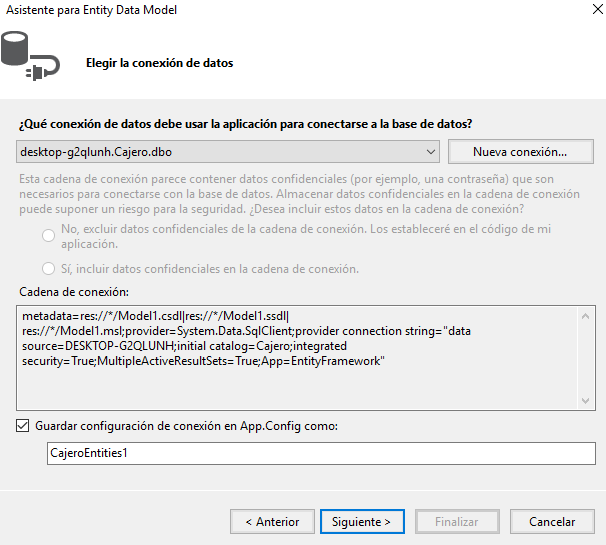
\includegraphics[width=8cm]{./Imagenes/img7}
		\end{center}
		\end{figure}
	\end{enumerate}

	\item Escribiendo consultas con el operador UNPIVOT
	\begin{enumerate}[a)]
	\item Paso 1: Crear y consultar la vista Sale.PivotCustGroups.\\
		-  Escribir la siguiente consulta para crear una vista llamada Sales.PivotCustGroups.\\
		\begin{figure}[H]
		\begin{center}
		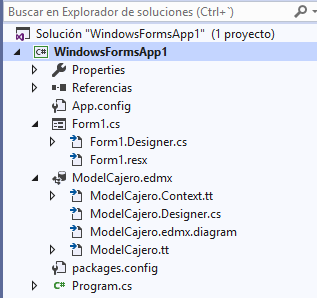
\includegraphics[width=8cm]{./Imagenes/img8}
		\end{center}
		\end{figure}
		-  Despues escribrir la siguiente consulta.
		\begin{figure}[H]
		\begin{center}
		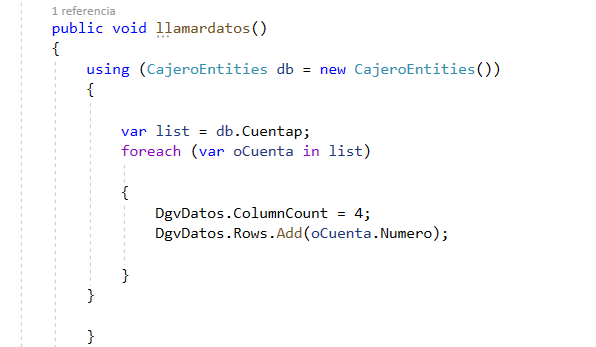
\includegraphics[width=5cm]{./Imagenes/img9}
		\end{center}
		\end{figure}
	\item Paso 2: Escriba una instruccion SELECT para recuperar una fila para cada pais y grupo de cliente.\\
		-  En el panel de consulta escribir la siguiente consulta.\\
		\begin{figure}[H]
		\begin{center}
		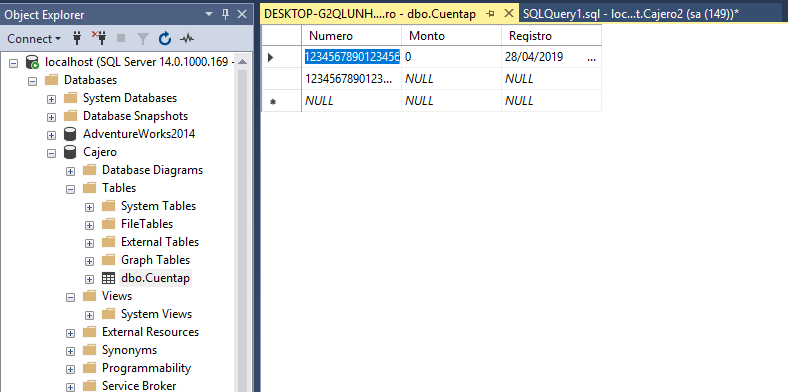
\includegraphics[width=7cm]{./Imagenes/img10}
		\end{center}
		\end{figure}
	\item Paso 3: Eliminar las vistas creadas.
		\begin{figure}[H]
		\begin{center}
		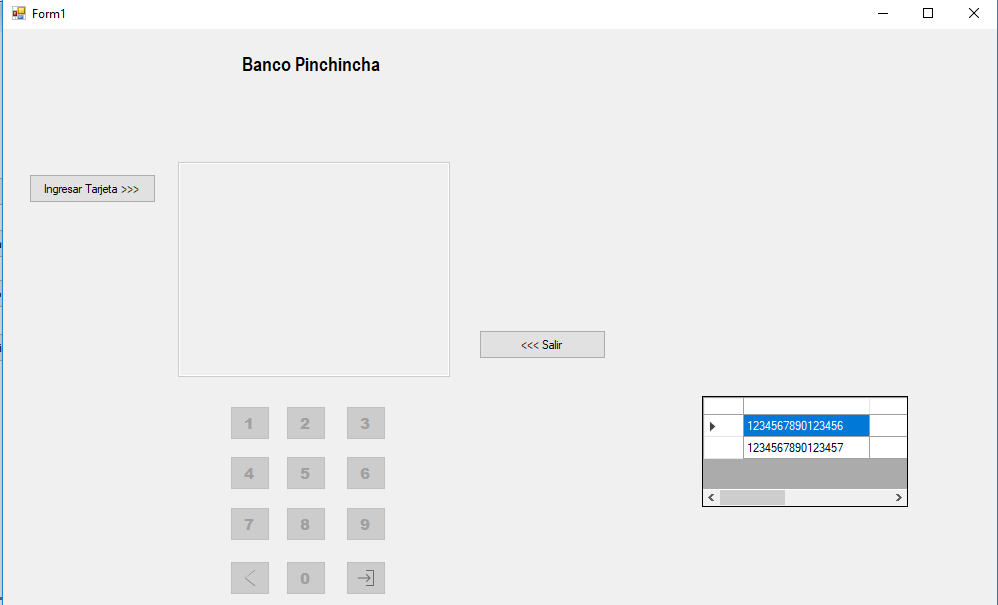
\includegraphics[width=6cm]{./Imagenes/img11}
		\end{center}
		\end{figure}
	\end{enumerate}



	\item Escribiendo consultas con las clausulas GROUPING SETS, CUBE, and ROLLUP.
	\begin{enumerate}[a)]
	\item Paso 1: Escriba una instruccion SELECT que use LA SUBCLAUSULA GROUPING SETS para devolver el número de
Clientes para diferentes conjuntos de agrupación.\\
		-  Escribir la siguiente consulta y ejecutar. 
		\begin{figure}[H]
		\begin{center}
		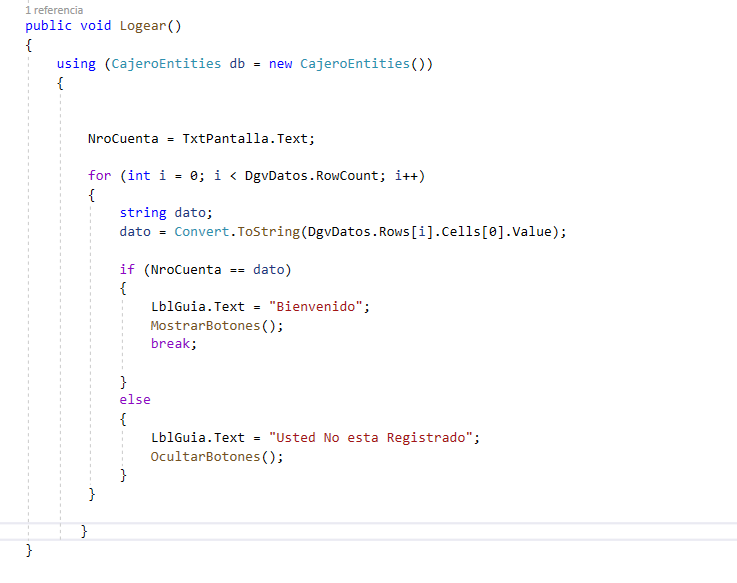
\includegraphics[width=7cm]{./Imagenes/img12}
		\end{center}
		\end{figure}
	\item Paso 2: Escriba una instruccion SELECT que use la subclausula CUBE para recuperar Grouping sets basados en valores de ventas anuales, mensuales y diarios.\\
		-  Escribir la siguiente consulta. 
		\begin{figure}[H]
		\begin{center}
		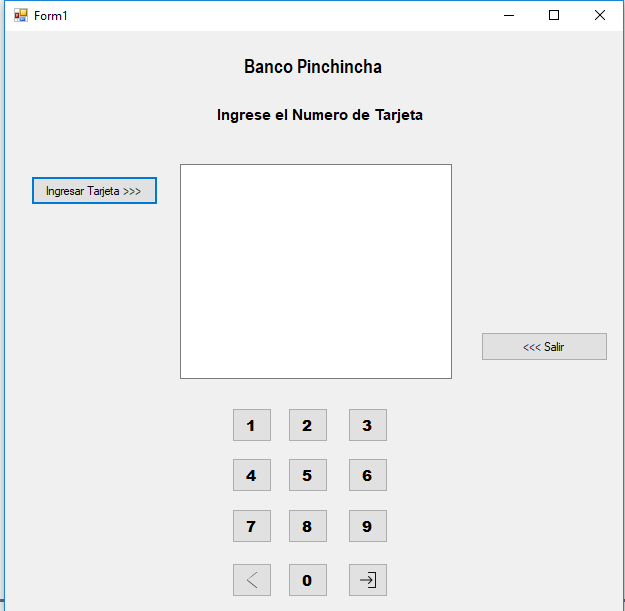
\includegraphics[width=7cm]{./Imagenes/img13}
		\end{center}
		\end{figure}
	\item Paso 3: Escriba la misma instruccion SELECT usando la subclausula ROLLUP.\\
		-  Escribir la siguiente consulta. 
		\begin{figure}[H]
		\begin{center}
		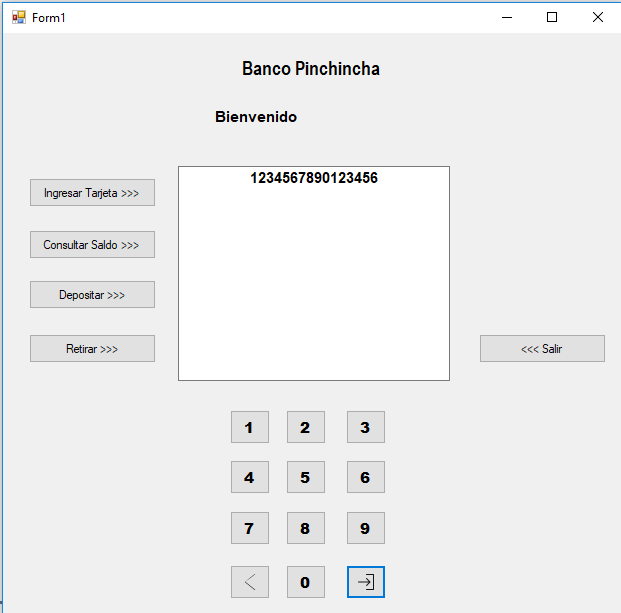
\includegraphics[width=7cm]{./Imagenes/img14}
		\end{center}
		\end{figure}
	\item Paso 4: Analizar el valor total de ventas por año y mes.\\
		-  Escribir la siguiente consulta y ejecutar. 
		\begin{figure}[H]
		\begin{center}
		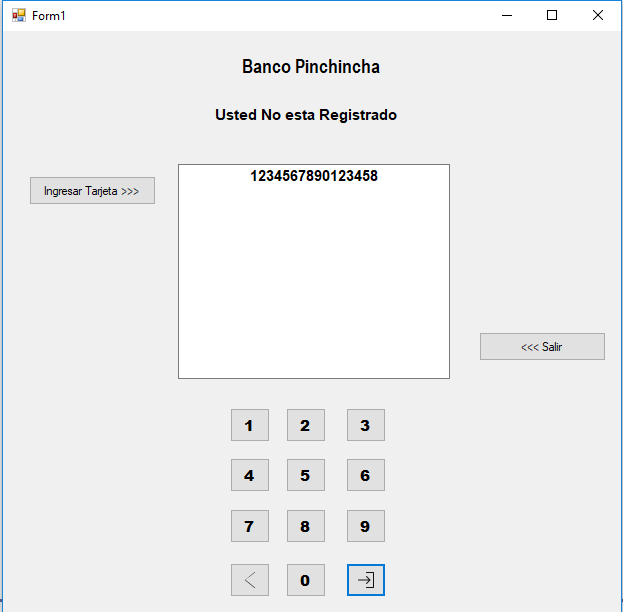
\includegraphics[width=7cm]{./Imagenes/img15}
		\end{center}
		\end{figure}
	\end{enumerate}
\end{enumerate}


\subsection{Pruebas}
\begin{enumerate}[1.]
	\item Escribiendo consultas con el operador PIVOT
	\begin{enumerate}[a)]
	\item Paso 1: Escribir una sentencia SELECT para recuperar el numero de clientes para un grupo especifico de clientes.\\
		-  Abrir el SQL Server Management Studio y conectar a la basa de datos (local) usando Windows.\\
		-  Usar la base de datos TSQL\\
		-  Ejecutar el siguiente codigo para crear una vista\\
		\begin{figure}[H]
		\begin{center}
		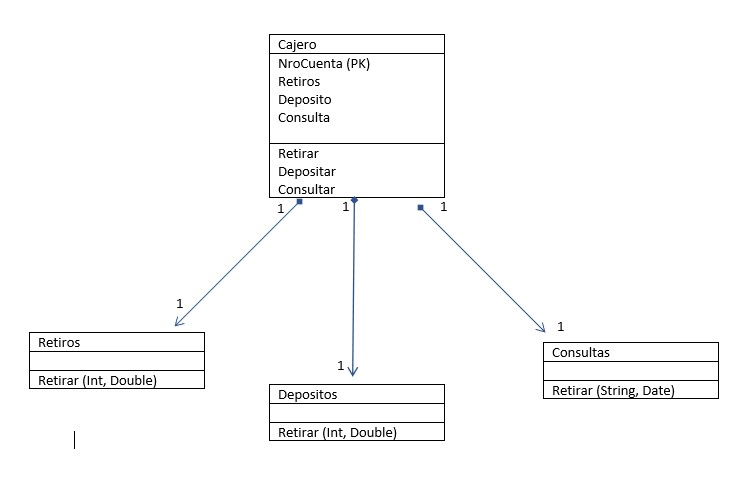
\includegraphics[width=8cm]{./Imagenes/img1}
		\end{center}
		\end{figure}
		-  En el panel de consulta, escribir la siguiente consulta.
		\begin{figure}[H]
		\begin{center}
		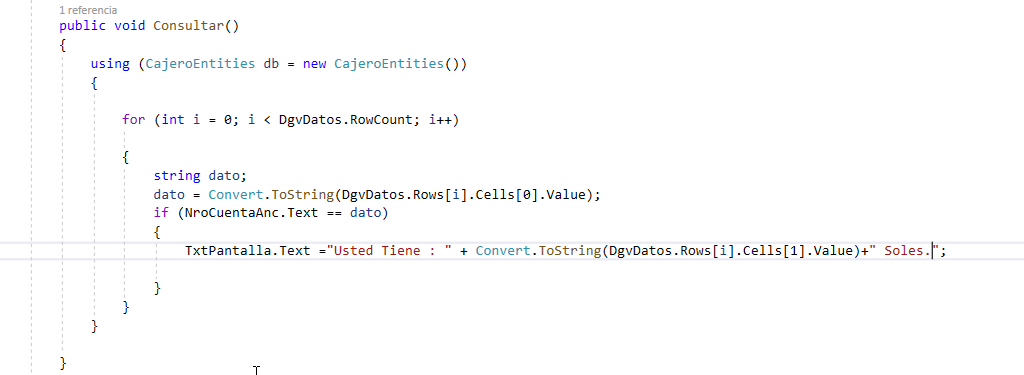
\includegraphics[width=6cm]{./Imagenes/img16}
		\end{center}
		\end{figure}
		-  Luego modificamos el codigo, aplicando el operador PIVOT.
		\begin{figure}[H]
		\begin{center}
		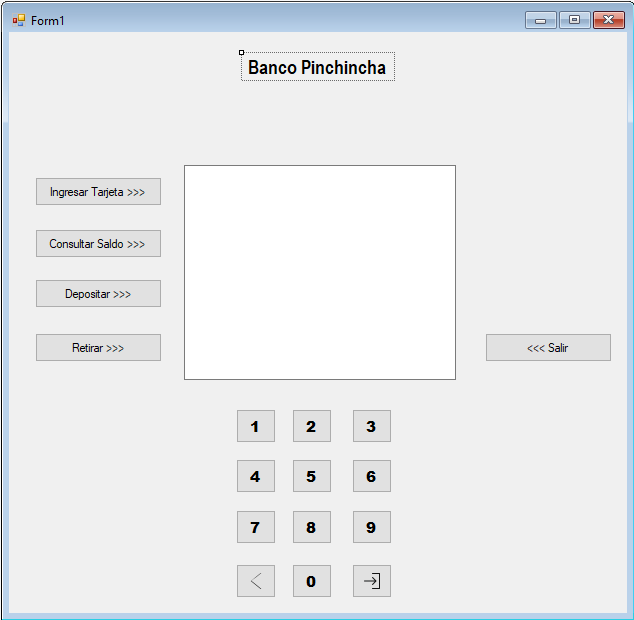
\includegraphics[width=6cm]{./Imagenes/img2}
		\end{center}
		\end{figure}
	\item Paso 2: Especifique el elemento de agrupacion para el operador PIVOT. \\
		-  Escribir la siguiente consulta para poder modificar la vista creada anteriormente, añadiendo 2 columnas adicionales. 
		\begin{figure}[H]
		\begin{center}
		\includegraphics[width=7cm]{./Imagenes/img3}
		\end{center}
		\end{figure}
		-  Escribir la siguiente consulta. 
		\begin{figure}[H]
		\begin{center}
		\includegraphics[width=6cm]{./Imagenes/img4}
		\end{center}
		\end{figure}
		-  Modificar la consulta para incluir columnas adicionales desde la vista. 
		\begin{figure}[H]
		\begin{center}
		\includegraphics[width=7cm]{./Imagenes/img5}
		\end{center}
		\end{figure}
	\item Paso 3: Use una expresion de tabla común (CTE) para especificar el elemnto de agrupacion para el operador PIVOT.\\
		-  Escribir la siguiente consulta y ejecutar. 
		\begin{figure}[H]
		\begin{center}
		\includegraphics[width=7cm]{./Imagenes/img6}
		\end{center}
		\end{figure}
	\item Paso 4: Escribe una instruccion SELECT para recuperar el monto total de ventas para cada cliente y categoria de producto.\\
		-  Escribir la siguiente consulta. 
		\begin{figure}[H]
		\begin{center}
		\includegraphics[width=8cm]{./Imagenes/img7}
		\end{center}
		\end{figure}
	\end{enumerate}
\end{enumerate}





